\chapter{سیستم پیشنهادی برای پرسش و پاسخ فارسی}
در این فصل سیستمی مناسب برای پاسخ‌دهی به مسائل شرح داده شده در فصل یک معرفی می‌شود. برای چنین سیستمی نیاز به یک پایگاه دانش می‌باشد تا اطلاعات مورد نیاز سیستم را فراهم نماید. برای فراهم کردن این اطلاعات از گراف دانش فارس‌بیس استفاده می‌شود. در ابتدای این فصل به معرفی این گراف دانش پرداخته شده و سپس بخش‌های دیگر سیستم معرفی می‌شوند.
\section{گراف دانش فارس‌بیس}
پایگاه دانش فارس‌بیس اولین پایگاه دانش طراحی شده مخصوص زبان فارسی می‌باشد.
فارس‌بیس از مدل فراداده‌ای چارچوب توصیف منابع برای ذخیره‌ی دانش استفاده می‌کند. برای اتصال به این پایگاه دانش و دریافت موجودیت پاسخ از زبان \lr{SPARQL}\footnote{\lr{SPARQL Protocol and RDF Query Language}} استفاده می‌شود.
برخلاف پایگاه‌های دانش انگلیسی زبان همانند \lr{Wikidata} که افراد مختلف بسیاری در گسترش آن کمک می‌کنند، در مورد پایگاه‌های فارسی زبان چنین اجتماع گسترده‌ای وجود ندارد و نمی‌توان به آن اتکا نمود؛ به همین سبب برای تولید پایگاه دانش فارس‌بیس از داده‌های خام متنی داخل وب استفاده شده و از طریق خزش وب دانش‌های موجود در آنها استخراج می‌گردند.
دانش‌های استخراج شده به صورت ترکیب‌های سه‌تایی در پایگاه فارس‌بیس ذخیره می‌شوند. این ترکیب‌های سه‌تایی شامل فاعل، مفعول و رابطه‌ی بین آنها می‌باشد. به عنوان مثال با استخراج این دانش که مادرید پایتخت کشور اسپانیا می‌باشد، سه‌تایی «اسپانیا، مادرید، پایتخت یک کشور» در پایگاه دانش ایجاد می‌شود.
سیستم استخراج‌کننده‌ی دانش فارس‌بیس دارای معماری‌ای با چندین لایه می‌باشد. استخراج دانش از ترکیب دو روش اصلی استخراج رابطه\footnote{\lr{Relation Extraction}} و استخراج اطلاعات\footnote{\lr{Information Extraction}} صورت می‌گیرد. برای استخراج رابطه از دو ماژول و برای استخراج اطلاعات از چهار ماژول مختلف توسعه‌یافته برای زبان فارسی استفاده می‌شود. همچنین در هر دو روش یک مرحله‌ی پیوند موجودیت‌ها\footnote{\lr{Entity Linking}} وجود دارد که فاعل و مفعول سه‌تایی مربوطه را ابهام‌زدایی کرده و به موجودیت‌های گراف دانش متصل می‌نماید. به موازات این مرحله، کانونی‌‌سازی\footnote{\lr{Canonicalization}} نیز انجام می‌شود. در مرحله‌ی کانونی‌سازی رابطه‌ی بین فاعل و مفعول در اطلاعات استخراج شده بدست آورده می‌شود. این مرحله فقط در روش استخراج اطلاعات مورد نیاز است. در نهایت، همه‌ی سه‌تایی‌های دانش کاندید که استخراج شده‌اند، پس از بازبینی و تایید شدن توسط یک متخصص انسانی به پایگاه دانش فارس‌بیس افزوده می‌شوند \cite{farsbase}.
سیستم پرسش و پاسخ فارسی مورد نظر از این پایگاه دانش استفاده می‌کند تا با داشتن رابطه و موجودیت مورد پرسش، سه‌تایی مربوطه در پایگاه دانش را پیدا کرده و پاسخ سوال را از آن استخراج نماید. برای انجام این کار نیاز است که سه زیرمسئله‌ی عنوان شده در فصل یک شامل تشخیص رابطه، تشخیص موجودیت‌ها و تولید کوئری توسط سیستم پاسخ داده شوند. برای پاسخ دادن به این زیرمسئله‌ها نیاز به مجموعه دادگان وجود دارد و با توجه به نبود دادگان برای پرسش و پاسخ فارسی، دادگان مورد نیاز در این پروژه تهیه شده‌اند. در ادامه با دادگان جمع‌آوری شده آشنا شده و سپس به شرح چگونگی انجام و حل سه زیرمسئله‌ی عنوان شده که سه بخش اصلی سیستم را تشکیل می‌دهند، می‌پردازیم.
\section{مجموعه دادگان}
به تعداد ۴۶ رابطه از گراف دانش فارس‌بیس استخراج شده است که آنها را در جدول \ref{tab:relations} مشاهده می‌نمایید. این روابط جز پرکاربردترین روابط در گراف دانش می‌باشند که توسط تهیه‌کنندگان گراف دانش فارسی مشخص شده‌اند.
\begin{longtable}{|c|c|}
	\hline
	\rowcolor{headerColor} 
	عنوان & شناسه
	\\ \hline پایتخت یک کشور & \lr{http://fkg.iust.ac.ir/ontology/capital}
	\\  واحد پول یک شرکت & \lr{http://fkg.iust.ac.ir/ontology/currency}
	\\  نوع حکومت یک کشور & \lr{http://fkg.iust.ac.ir/ontology/governmentType}
	\\  زبان رسمی یک کشور & \lr{http://fkg.iust.ac.ir/ontology/language}
	\\  مساحت یک کشور & \lr{http://fkg.iust.ac.ir/ontology/areaTotal}
	\\  جمعیت یک کشور & \lr{http://fkg.iust.ac.ir/ontology/populationTotal}
	\\  کارگردان یک فیلم & \lr{http://fkg.iust.ac.ir/ontology/director}
	\\  بازیگران یک فیلم & \lr{http://fkg.iust.ac.ir/ontology/starring}
	\\  نویسنده یک فیلم & \lr{http://fkg.iust.ac.ir/ontology/writer}
	\\  آهنگساز یک فیلم & \lr{http://fkg.iust.ac.ir/ontology/musicComposer}
	\\  بودجه یک فیلم & \lr{http://fkg.iust.ac.ir/ontology/budget}
	\\  میزان فروش یک فیلم & \lr{http://fkg.iust.ac.ir/ontology/gross}
	\\  ترکیبات یک غذا & \lr{http://fkg.iust.ac.ir/ontology/ingredient}
	\\  آثار یک شخص & \lr{http://fkg.iust.ac.ir/ontology/notableWork}
	\\  باشگاه های یک ورزشکار & \lr{http://fkg.iust.ac.ir/ontology/club}
	\\  محل تحصیل یک شخص & \lr{http://fkg.iust.ac.ir/ontology/almaMater}
	\\  استاندار یک استان & \lr{http://fkg.iust.ac.ir/ontology/governorGeneral}
	\\  محل دفن یک شخص & \lr{http://fkg.iust.ac.ir/ontology/deathPlace}
	\\  تاریخ مرگ یک شخص & \lr{http://fkg.iust.ac.ir/ontology/deathDate}
	\\ فرزندان یک شخص & \lr{http://fkg.iust.ac.ir/ontology/child}
	\\  سرمربی یک تیم ورزشی & \lr{http://fkg.iust.ac.ir/ontology/property}
	\\  مرکز یک استان & \lr{http://fkg.iust.ac.ir/ontology/capital}
	\\  کارگردان یک سریال تلویزیونی & \lr{http://fkg.iust.ac.ir/ontology/director}
	\\  بازیگران یک سریال تلویزیونی & \lr{http://fkg.iust.ac.ir/ontology/starring}
	\\  نویسنده یک سریال تلویزیونی & \lr{http://fkg.iust.ac.ir/ontology/author}
	\\  قد یک ورزشکار & \lr{http://fkg.iust.ac.ir/ontology/Person/height}
	\\  مساحت یک دریا یا اقیانوس & \lr{http://fkg.iust.ac.ir/ontology/areaTotal}
	\\  دوره ساخت یک مکان یا بنا & \lr{http://fkg.iust.ac.ir/ontology/era}
	\\  همسر یک شخص & \lr{http://fkg.iust.ac.ir/ontology/spouse}
	\\  محل یک مکان یا بنا & \lr{http://fkg.iust.ac.ir/ontology/county}
	\\  ملیت یک شخص & \lr{http://fkg.iust.ac.ir/ontology/nationality}
	\\ نویسنده کتاب & \lr{http://fkg.iust.ac.ir/ontology/author}
	\\  ناشر کتاب & \lr{http://fkg.iust.ac.ir/ontology/publisher}
	\\  پیش شماره & \lr{http://fkg.iust.ac.ir/ontology/areaCode}
	\\  مساحت & \lr{http://fkg.iust.ac.ir/ontology/areaTotal}
	\\  جمعیت & \lr{http://fkg.iust.ac.ir/ontology/populationTotal}
	\\  شهردار & \lr{http://fkg.iust.ac.ir/ontology/leaderName}
	\\  محصولات شرکت & \lr{http://fkg.iust.ac.ir/ontology/service}
	\\  سایت یک شرکت & \lr{http://xmlns.com/foaf/0.1/homepage}
	\\ مدیر عامل شرکت & \lr{http://fkg.iust.ac.ir/ontology/ceo}
	\\  درامد & \lr{http://fkg.iust.ac.ir/ontology/revenue}
	\\  پلاک & \lr{http://fkg.iust.ac.ir/ontology/vehicleCode}
	\\  بزرگترین شهر یک کشور & بزرگترین\lr{\_}شهر\lr{http://fkg.iust.ac.ir/ontology/}
	\\  وزیر یک وزارتخانه & \lr{http://fkg.iust.ac.ir/ontology/leader}
	\\  تعداد کارکنان یک شرکت یا ارگان & \lr{http://fkg.iust.ac.ir/ontology/numberOfStaff}
	\\  نام ورزشگاه یک تیم ورزشی & \lr{http://fkg.iust.ac.ir/ontology/ground}
	\\ \hline	 	
	\caption{عنوان روابط و شناسه آنها در گراف دانش فارس‌بیس}
	\label{tab:relations}
\end{longtable}
\noindent به ازای هر کدام از روابط فوق مجموعه‌ای از جملات الگو به منظور آموزش به مدل‌ها در فایل \lr{rel\_q.csv} جمع‌آوری شده‌اند. تعدادی از الگوهای رابطه‌ی "پایتخت یک کشور" را در جدول \ref{tab:templates_capital} مشاهده می‌نمایید.
\begin{table}[h]
	\centering
	\def\arraystretch{1.6}
	\begin{tabular}{|c|}
		\hline
		پایتخت کشور ررر چه نام دارد
		\\پایتخت ررر چه نام دارد
		\\شهر ششش پایتخت کدام کشور است
		\\نام کشوری که شهر ششش پایتخت آن است چیست
		\\پایتخت کشور ررر چه می‌باشد
		\\ \hline	 
	\end{tabular}	
	\caption{نمونه‌هایی از جملات الگو برای رابطه‌ی "پایتخت یک کشور"}
	\label{tab:templates_capital}
\end{table}
\\در جملات الگو به جای موجودیت‌ها نماد آنها جایگزین شده است. به عنوان مثال در جملات جدول \ref{tab:templates_capital} "ررر" نماد موجودیت کشور و "ششش" نماد موجودیت شهر می‌باشد. هدف از انتخاب این نمادها اطمینان از عدم وجود آن‌ها در واژگان زبان فارسی می‌باشد. به ازای هر یک از این نمادها تعدادی موجودیت مرتبط از پایگاه دانش فارس‌بیس استخراج شده و در جملات الگو قرار داده می‌شوند و از این جملات تولید شده برای آموزش مدل‌ها استفاده می‌شود.

\section{تشخیص رابطه}
این بخش از سیستم وظیفه‌ی تشخیص رابطه‌ی موجود در سوال مورد پرسش کاربر را دارد که بوسیله‌ی یک دسته‌بند قابل انجام است. به این منظور دسته‌بندهای ماشین بردار پشتیبان و شبکه عصبی پیچشی که در فصل دوم با آن آشنا شدیم بکار گرفته شده‌اند. در این بخش به طور مختصر چگونگی استفاده از این دسته‌بندها برای این سیستم توضیح داده می‌شود. این دسته‌بندها در پکیج\footnote{\lr{Package}} \lr{classifiers} پیاده‌سازی شده‌اند. در این پکیج یک کلاس انتزاعی\footnote{\lr{Abstract}} پیاده شده و کلاس‌های مربوط به مدل‌های ماشین بردار پشتیبان و شبکه عصبی پیچشی از آن ارث‌بری می‌کنند. برای استفاده از این دسته‌بندها نیاز به یک مرحله پیش‌پردازش روی سوالات ورودی می‌باشد که در ادامه به شرح آن می‌پردازیم.

\subsection{‌تعبیه‌سازی کلمات}
برای استفاده از دسته‌بندها ابتدا باید سوالات ورودی به بردارهایی نگاشت شوند و از آن بردارها به عنوان ورودی دسته‌بند استفاده شود. برای این منظور از چهار روش تعبیه‌سازی\footnote{\lr{Embedding}} کلمات شامل کوله‌ی کلمات\footnote{\lr{Bag of Words}} که آنرا با نماد \lr{BOW} نمایش می‌دهیم، روش \lr{TF-IDF}\footnote{\lr{Term Frequency-Inverse Document Frequency}} و یک مدل \lr{word2vec} استفاده شده است. روش چهارم استفاده از همان مدل \lr{word2vec} به صورت وزن‌دار است که وزن‌های آن همان مقادیر معکوس فراوانی متن استفاده شده در روش \lr{TF-IDF} برای هر کلمه می‌باشد.
این مدل‌ها در فایل \lr{feature\_extractor.py} پیاده‌سازی شده‌اند. \\
مدل ماشین بردار پشتیبان با هر چهار روش فوق و مدل شبکه عصبی پیچشی با روش \lr{word2vec} بدون وزن قابل استفاده بوده و مورد آزمایش قرار گرفته‌اند.

\subsection{دسته‌بند ماشین بردار پشتیبان‌‌}
ماشین بردار پشتیبان یک روش یادگیری با نظارت است که از آن برای دسته‌بندی و رگرسیون\footnote{\lr{Regression}} می‌توان استفاده کرد. مبنای کار ماشین بردار پشتیبان دسته‌بندی خطی داده‌ها است به طوری که خطی به عنوان تقسیم‌کننده استفاده شود که بیشترین حاشیه اطمینان را داشته باشد. حل این مسئله منجر به یک مسئله‌ی بهینه‌سازی برنامه‌ریزی درجه دوم\footnote{\lr{Quadratic Programming}} مقید می‌گردد.
همچنین می‌توان از این ماشین برای دسته‌بندی داده‌های جدایی‌ناپذیر خطی هم استفاده کرد؛ به طوریکه قبل از استفاده از ماشین بردار پشتیبان، داده‌ها توسط تابعی تحت عنوان تابع هسته\footnote{\lr{Kernel}} به فضایی دیگر انتقال داده می‌شوند که در آن فضا جدایی‌پذیر خطی باشند. یک نمونه از این انتقال در شکل \ref{fig:svm-kernel} نمایش داده شده‌ است.\\
در این سیستم از تابع پایه شعاعی\footnote{\lr{Radial Basis Function (RBF)}} به عنوان هسته‌ی این دسته‌بند استفاده می‌شود.

\begin{figure}[t!]
	\centering
	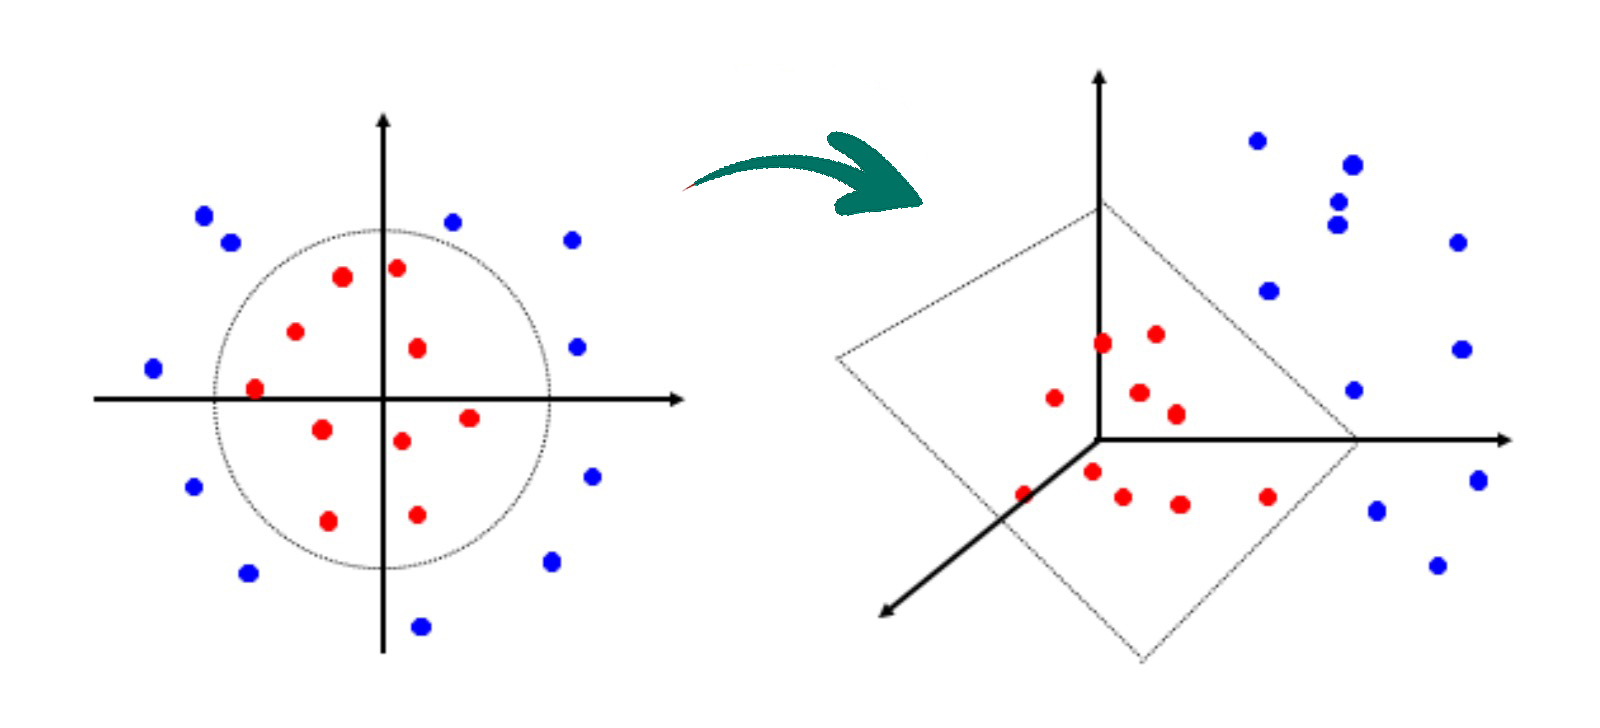
\includegraphics[scale=0.25]{figures/svm-kernel.jpeg}
	\caption[تابع هسته‌ی دایره‌ای در ماشین بردار پشتیبان]{جداپذیرخطی کردن داده‌ها با انتقالشان از فضای دوبعدی به سه‌بعدی بوسیله‌ی یک هسته‌ی تابع پایه شعاعی}
	\label{fig:svm-kernel}
\end{figure}

\subsection{دسته‌بند شبکه عصبی پیچشی}
پیاده‌سازی این شبکه توسط کتابخانه‌ی متن‌باز \lr{Keras} انجام شده است. این شبکه یک جمله را به صورت یک بردار تک‌بعدی دریافت می‌کند که هر خانه‌ی این آرایه کد کلمه‌ی متناطر در لیست واژگان را مشخص می‌کند. خروجی شبکه نیز یک بردار تک‌بعدی به طول ۴۶ می‌باشد که احتمال هر رابطه را برای جمله‌ی ورودی مشخص می‌نماید. همانطور که در شکل  \ref{fig:cnn-model} مشاهده می‌کنید، اولین لایه‌ی شبکه یک لایه‌ی تعبیه‌ساز است که از مدل \lr{word2vec} توضیح داده شده استفاده می‌کند تا هر کلمه را به بردار متناسب آن نگاشت کند.
لایه‌ی سوم که هسته‌ی این شبکه می‌باشد در ادامه توضیح داده خواهد شد. 
در ادامه دو لایه شبکه‌ از نورون‌ها (\lr{Dense}) همراه با تابع فعال‌ساز\footnote{\lr{Activation}} \lr{ReLU} حضور دارند که در نهایت بوسیله‌ی یک لایه‌ی فعال‌ساز \lr{Softmax} احتمالات هر یک از کلاس‌ها که خروجی دسته‌بند است تولید می‌شود. در میان این لایه‌ها دو لایه‌ی حذفی تصادفی\footnote{\lr{Dropout}} حضور دارند که فقط هنگام آموزش فعال هستند و هدف آنها کاهش بیش‌بردازش\footnote{\lr{Overfitting}} در هنگام آموزش می‌باشد. \\
هسته‌ی این شبکه، یک شبکه‌ی پیچشی است که وظیفه‌ی آن تشخیص الگوهای جملات ورودی است. همانطور که در شکل \ref{fig:cnn-model-core} مشاهده می‌کنید، این شبکه از سه قسمت موازی مشابه تشکیل می‌شود. در هر قسمت ابتدا یک لایه شبکه‌ی کانولوشن وجود دارد که در هر کدام از آنها ظرفیت لازم برای تشخیص ۱۵۰ فیلتر در نظر گرفته شده است. اما اندازه‌ی هسته یا فیلتر آنها متفاوت بوده و طول آن در هر کدام به ترتیب سه، چهار و پنج کلمه در نظر گرفته شده است. در ادامه در هر سه قسمت مقادیر به یک لایه‌ی ادغام حداکثر\footnote{\lr{Max Pooling}} به طول دو وارد شده و سپس تمامی مقادیر بهم الحاق شده و از این شبکه‌ی داخلی خارج می‌شوند \cite{yoon2014conv}.
\\از تابع هزینه‌ی \lr{Categorical Cross-Entropy} برای آموزش این شبکه استفاده شده است.
\begin{figure}
	\centering
	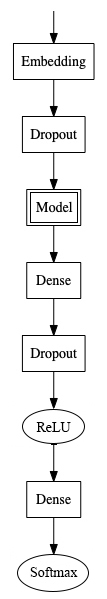
\includegraphics[width=3cm]{figures/cnn/cnn-model.jpg}
	\caption[لایه‌های دسته‌بند شبکه عصبی پیچشی]{لایه‌های دسته‌بند شبکه عصبی پیچشی}
	\label{fig:cnn-model}
\end{figure}

\begin{figure}
	\centering
	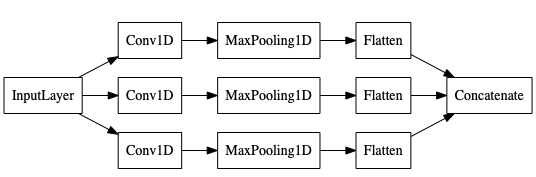
\includegraphics[width=15cm]{figures/cnn/cnn-model-core.jpg}
		\caption[لایه‌های هسته‌ی دسته‌بند شبکه عصبی پیچشی]{لایه‌های هسته‌ی دسته‌بند شبکه عصبی پیچشی}
	\label{fig:cnn-model-core}
\end{figure}

\section{تشخیص موجودیت‌ها}
برای تشخیص موجودیت‌های جمله‌ی مورد پرسش دو امکان در این سیستم موجود است. امکان اول استفاده از رابط‌های برنامه‌نویسی کاربردی\footnote{\lr{API}} موجود در سیستم فارس‌بیس است که امکان تشخیص موجودیت‌های موجود در جمله را دارند. امکان دوم استفاده از کتابخانه‌ی تشخیص‌دهنده موجودیت‌های نام‌دار\footnote{\lr{Named-Entity Recognition}} پیاده‌سازی شده در آزمایشگاه پردازش زبان طبیعی امیرکبیر است که در پکیج \lr{NER\_module} موجودند. 
در این سیستم خروجی هر دو روش گرفته شده و از آنهایی که گره‌ی مرتبط در گراف فارس‌بیس دارند استفاده می‌شود. روندهای مربوط به این قسمت در فایل \lr{NER\_provider} قابل مشاهده می‌باشند.
در ادامه خروجی این دو روش را برای جمله‌ی "پایتخت کشور آلمان کجاست" مشاهده می‌کنید. خروجی اول مربوط به رابط برنامه‌نویسی فارس‌بیس و خروجی دوم مربوط به کتابخانه‌ی تشخیص‌دهنده می‌باشد:
\begin{flushleft}
\lr{['Beginning :Thing', 'Beginning :Country', 'Inside :Country', 'Outside']}\\
\lr{['o', 'o', 'b-loc', 'o'].}
\end{flushleft}
\section{تولید کوئری}
رابطه و موجودیت‌ تشخیص داده شده توسط بخش‌های دیگر سیستم که توضیح داده شدند، در این بخش استفاده شده و کوئری مناسب تولید می‌شود. از آنجا که پایگاه دانش از یک گراف جهت‌دار ساخته شده است، موجودیت سوال می‌تواند در ابتدا و یا انتهای رابطه باشد. بر همین اساس کوئری ارسالی به دو صورت می‌تواند ساخته شود که هر دو قالب را در ادامه مشاهده می‌کنید:

\begin{multicols}{2}
	\begin{LTR}
		\begin{verbatim}
		select distinct(?o) where {
		<‌entity_uri> <relatoin_uri> ?o.
		}
		\end{verbatim}
	\end{LTR}
	\columnbreak
	
	\begin{LTR}
		\begin{verbatim}
		select distinct(?o) where {
		?o <relation_uri> <entity_uri>.
		}
		\end{verbatim}
	\end{LTR}
\end{multicols}
به عنوان مثال برای پرسش "پایتخت آلمان کجاست" موجودیت "آلمان" و رابطه‌ی "پایتخت یک کشور" بدست آورده شده‌اند. با استفاده از این اطلاعات و بدست آوردن جهت رابطه در این سوال کوئری زیر تولید می‌شود:
\begin{LTR}
	\noindent \lr{select distinct(?o) where }$\{$
	\\\lr{<http://fkg.iust.ac.ir/resource/}آلمان\lr{>}
	\lr{<http://fkg.iust.ac.ir/ontology/capital>}
	\lr{?o.}
	\\$\}$
\end{LTR}
اگر برای پرسش ورودی چندین رابطه با احتمال بالا و یا چندین موجودیت تشخیص داده شود، از ترکیب آنها چندین کوئری ساخته شده و در مرحله‌ی ارسال از همه‌ی آنها استفاده می‌شود و چندین پاسخ برای کاربر بازگردانده می‌شود. 
